\documentclass[11pt]{article}

\usepackage{float}
\usepackage{hyperref}
\usepackage{fullpage}
\usepackage{verbatim}
\usepackage{moreverb}
\usepackage{graphicx}
\usepackage{parskip}
\usepackage{amsmath}
\usepackage[toc,page]{appendix}
\graphicspath{{images/}}

\usepackage{minted}
\let\verbatiminput=\verbatimtabinput
\def\verbatimtabsize{4\relax}

\begin{document}
\title{EE 241B HW2 Writeup}

\author{Vighnesh Iyer}
\date{}
\maketitle

\tableofcontents

\section{Extracting and Simulating a Synthesized Design}
We start with an already placed and routed 4-bit decoder and we go through the flow of extracting parasitics, running LVS, and running SPICE simulations of the extracted schematic.

\subsection{Delay of a Path}
For the path from A[2] to Z[15] rise, what is the delay measured by IC Compiler, SPICE simulation without extracted parasitics, and SPICE simulation with parasitics?

\begin{itemize}
	\item IC Compiler: 0.08215 ns
	\begin{figure}[H]
		\centerline{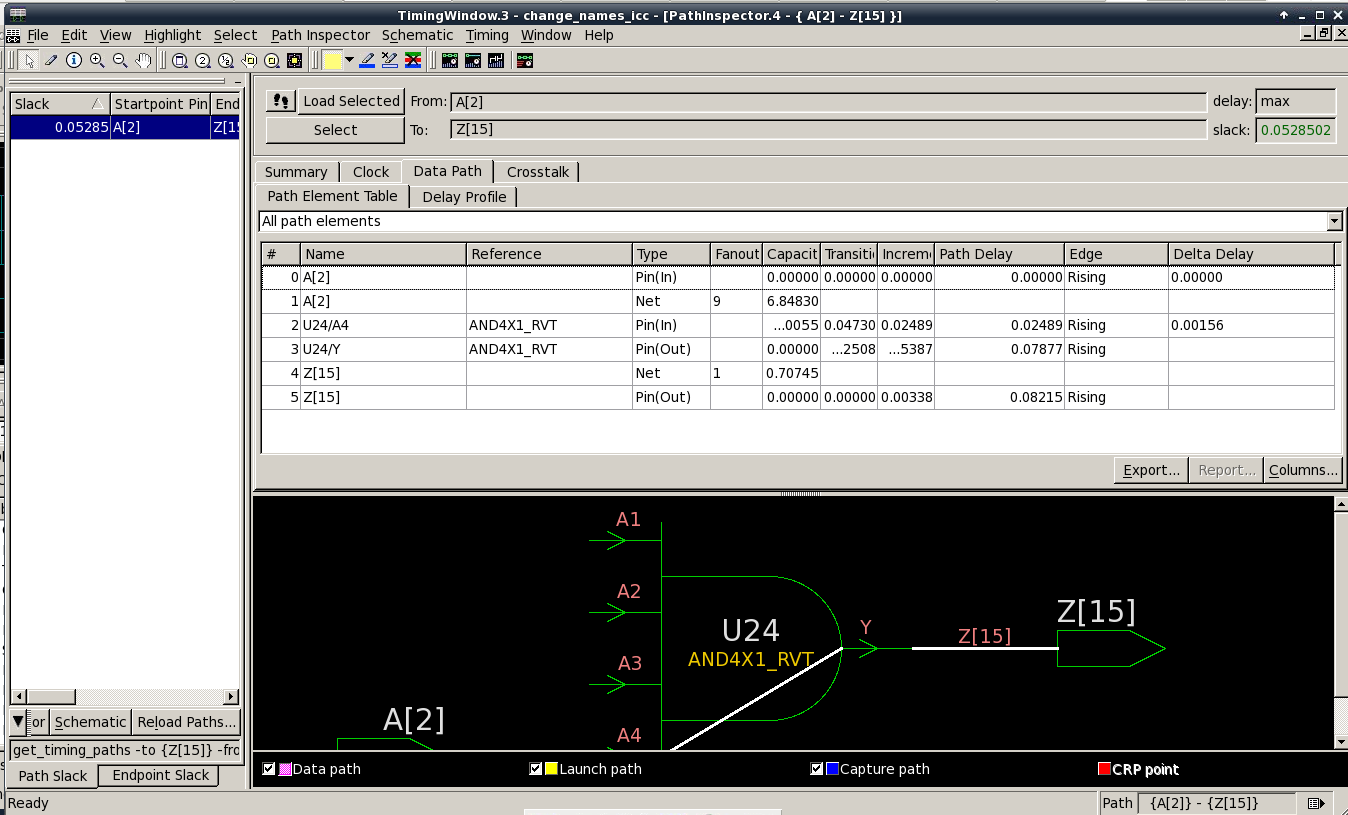
\includegraphics[height=6cm]{icc_path_delay.png}}
	\end{figure}

	\item SPICE without parasitics
	\begin{figure}[H]
		\centerline{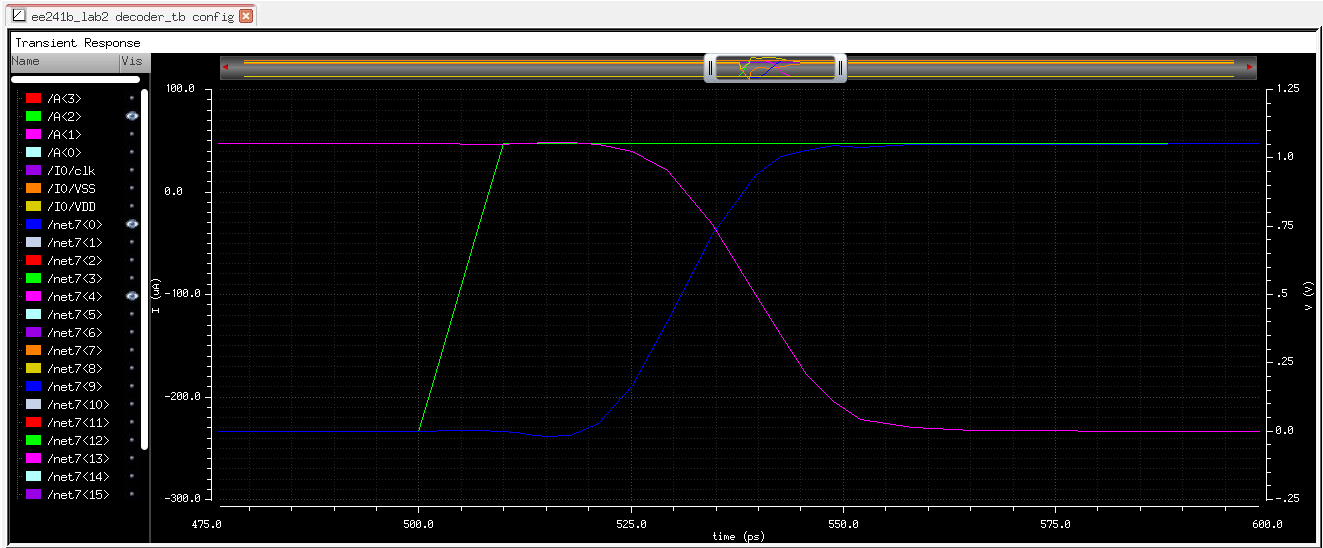
\includegraphics[height=6cm]{spice_path_delay.png}}
	\end{figure}
	
	\item SPICE with parasitics
\end{itemize}

\subsection{ICC Critical Path + Special Path}
We display the critical path in ICC and also highlight the special path noted above from the rise of A[2] to the rise of Z[15].

The critical path is from rising A[3] to falling Z[5], and it has a negative slack of -0.00263 ns. It is highlighted in red. The special path above is highlighted in yellow. 

\begin{figure}[H]
	\centerline{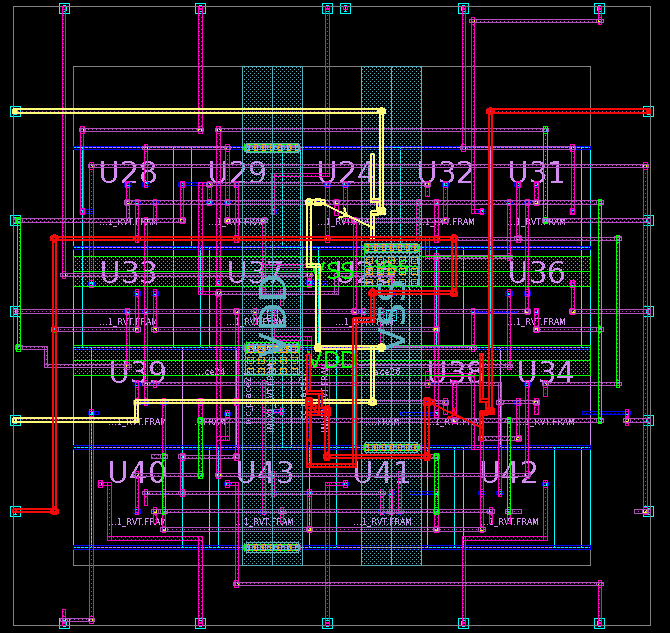
\includegraphics[height=8cm]{icc_critical_path.png}}
\end{figure}

\subsection{Power Estimate Accuracy Analysis}
We run the functional testbench that counts from A=0000 to A=1111 and report the power measured by Primetime, the SPICE simulation, and the mixed-signal simulation.

\begin{itemize}
	\item Primetime
	\item SPICE
	\item Mixed-Signal
\end{itemize}

\subsection{Voltage Scaling Power Estimates}
We run the mixed-signal simulation at 1.05V, 0.8V, 0.6V, and 0.4V and measure the average power for each voltage. We then convert average power to energy/op in terms of J/op and uW/Mhz. These results are compared to the theoretically predicted active energy savings for voltage scaling based on the 1.05V result.

The clock period will have to increase for lower supply voltages to compensate for increased delay.

\section{FF and Latch Based Timing}

\section{Variability and Timing Simulations}

\newpage
\appendix
\section{PMOS/NMOS DC Characterization SPICE Sim} \label{dc_characterization_spice}


\end{document}